\documentclass[conference]{IEEEtran}
\IEEEoverridecommandlockouts

\usepackage{iftex}
\ifXeTeX % local XeTeX builds: use a Times clone so the layout matches pdfLaTeX on Overleaf
  \usepackage{fontspec}
  \setmainfont{texgyretermes}[Extension=.otf, UprightFont=*-regular, BoldFont=*-bold,
    ItalicFont=*-italic, BoldItalicFont=*-bolditalic]
\fi
\usepackage{cite}
\usepackage{amsmath,amssymb,amsfonts}
\usepackage{graphicx}
\usepackage{booktabs}
\usepackage{array}
\usepackage{xcolor}
\usepackage{url}
\usepackage{algorithm}
\usepackage{algpseudocode}
\usepackage{tikz}
\usetikzlibrary{positioning,arrows.meta,fit,calc,backgrounds}

\graphicspath{{figures/}}

% Diagram styles
\tikzset{
  blk/.style={draw, rounded corners=2pt, align=center, font=\scriptsize, minimum height=8.5mm, inner sep=2pt, fill=white},
  sDATA/.style={blk, fill=blue!7},
  sPROC/.style={blk, fill=orange!10},
  sNET/.style={blk, fill=green!9},
  sOUT/.style={blk, fill=red!8},
  arr/.style={-{Stealth[length=1.6mm]}, semithick},
  lane/.style={draw=gray!60, dashed, rounded corners=3pt, inner sep=4pt},
  lanelabel/.style={font=\scriptsize\itshape, text=gray!70!black, anchor=south west},
}

\newcommand{\cmark}{\checkmark}
\newcommand{\xmark}{$\times$}

\begin{document}

\title{A Standards-Compliant, Inter-Patient Evaluated Lightweight ECG Arrhythmia Classifier for Resource-Constrained Embedded Deployment}

\author{
\IEEEauthorblockN{Nabarun Dey}
\IEEEauthorblockA{School of Computer Engineering\\
Manipal Institute of Technology\\
MAHE, Manipal, India\\
Reg. No. 240911236\\
{\footnotesize nabarun.mitmpl2024@learner.manipal.edu}}
\and
\IEEEauthorblockN{Jerome Varghese}
\IEEEauthorblockA{School of Computer Engineering\\
Manipal Institute of Technology\\
MAHE, Manipal, India\\
Reg. No. 240911430\\
{\footnotesize jerome.mitmpl2024@learner.manipal.edu}}
\and
\IEEEauthorblockN{S. Durgaprasad}
\IEEEauthorblockA{School of Computer Engineering\\
Manipal Institute of Technology\\
MAHE, Manipal, India\\
Reg. No. 240911023\\
{\footnotesize durgaprasad.mitmpl2024@learner.manipal.edu}}
}

\maketitle

\begin{abstract}
Only 5 of 122 recent ECG arrhythmia studies simultaneously follow the AAMI EC57 standard, test on patients unseen during training, and assess embedded feasibility. We present a lightweight one-dimensional convolutional neural network (1D-CNN) that meets all three criteria. Each MIT-BIH heartbeat is classified into the five AAMI classes from its single-lead morphology and eight RR-interval features measured relative to the patient's own rhythm. Training uses the DS1 records only; every design choice is made on a patient-wise DS1 hold-out, and the DS2 records are the inter-patient test set. The final model is an ensemble of three 4,974-parameter networks quantized to 8-bit integers. On DS2 it reaches 87.30\% accuracy, an SVEB sensitivity of 74.46\% (positive predictivity 33.43\%), and a VEB sensitivity of 92.89\% (positive predictivity 92.71\%). The ensemble needs 15.1~KB of INT8 weights, 0.76~million multiply-accumulates per beat and about 3.9~KB of peak activation memory, under 1\% of the 520~KB SRAM of an ESP32-WROOM-32E. Quantization costs 0.1 points of accuracy. Most SVEB false alarms (86.5\%) come from five patients with atrial fibrillation or AV block.
\end{abstract}

\begin{IEEEkeywords}
ECG, arrhythmia classification, AAMI EC57, inter-patient evaluation, 1D-CNN, quantization, embedded systems, TinyML
\end{IEEEkeywords}

%=====================================================================
\section{Introduction}
%=====================================================================
Cardiovascular diseases are the leading cause of death worldwide, accounting for an estimated 19.8~million deaths in 2022~\cite{who2025cvd}. Arrhythmias are a key indicator of cardiac health, and the electrocardiogram (ECG) is the standard non-invasive tool to detect them. Wearable patches, Holter monitors and loop recorders make continuous monitoring outside hospitals practical, which creates demand for automatic classifiers that run directly on small, low-power devices~\cite{silva2026review,demeloribeiro2022quantized,busia2025tiny}.

Many deep-learning studies report accuracies above 95\%~\cite{xiao2023review}, but these figures often do not transfer to deployment, for two reasons. First, the AAMI EC57 standard~\cite{aami2012ec57} defines beat classes and metrics but not the data partition. Many studies place beats of the same patient in both training and test sets (\emph{intra-patient}), so a model can memorize patient-specific morphology. Under the \emph{inter-patient} paradigm of de Chazal et al.~\cite{dechazal2004automatic}, training and test patients are disjoint, and performance drops sharply for the clinically important minority classes. Second, many accurate models exceed microcontroller memory and energy budgets, and few papers measure this. Silva et al.~\cite{silva2026review} call these requirements the E3C criteria: AAMI compliance, inter-patient evaluation and embedded feasibility. Of 122 studies, 68 (55.7\%) follow AAMI, 37 (30.3\%) use an inter-patient split, 38 (31.1\%) assess embedded feasibility, and only 5 (4.1\%) meet all three.

This project addresses that gap. We (i)~design a compact AAMI-compliant 1D-CNN with patient-relative RR features, trained on DS1 and tested on DS2 with every choice made on a patient-wise hold-out; (ii)~compress it to INT8 and measure size, operations and peak memory against an ESP32-WROOM-32E budget; (iii)~combine three INT8 networks into an ensemble that removes large seed-to-seed variance; and (iv)~analyze the remaining errors and freeze the final model with checksums before its single test-set evaluation.

%=====================================================================
\section{Literature Survey}
%=====================================================================
\emph{Standards and protocol.} AAMI EC57~\cite{aami2012ec57} groups MIT-BIH beat types into normal (N), supraventricular ectopic (SVEB), ventricular ectopic (VEB), fusion (F) and unknown (Q). It recommends excluding paced records and reporting sensitivity (Se), positive predictivity (+P) and false positive rate (FPR). MIT-BIH~\cite{moody2001impact,goldberger2000physiobank} holds 48 half-hour two-lead recordings at 360~Hz from 47 patients. Surveys~\cite{xiao2023review,luz2016survey} agree that intra- and inter-patient results are not comparable. About 89\% of beats are normal, so per-class Se and +P are the informative metrics.

\emph{Accuracy-oriented models.} Kiranyaz et al.~\cite{kiranyaz2016realtime} showed that compact 1D-CNNs classify beats in real time. Large models such as the residual network of Ribeiro et al.~\cite{ribeiro2020automatic} or the transformer of Hu et al.~\cite{hu2022transformer} (about 20~MB) show what unconstrained models achieve, but they are not microcontroller-class.

\emph{Edge-oriented models.} DL-LAC~\cite{sakib2021ultraedge} measured time and memory on virtualized microcontrollers. Seitanidis et al.~\cite{seitanidis2022edge} deployed a 2D-CNN on a Jetson Nano with a random 80/20 split. De Melo Ribeiro et al.~\cite{demeloribeiro2022quantized} quantized a 1D-CNN to 93~kB under an intra-patient protocol. Busia et al.~\cite{busia2025tiny} ran a 6,649-parameter INT8 transformer on GAP9 (4.28~ms, 0.09~mJ), again with a shuffled split. Kim et al.~\cite{kim2024ultraedge} met all three criteria with a 25~kB model using 118~kB RAM on a Cortex-M4, but used a custom subject partition. Farag~\cite{farag2023tiny} reported an inter-patient 15~kB CNN on a Raspberry Pi with 12--24~MB runtime memory. Saha Tchinda and Tchiotsop~\cite{sahatchinda2025lightweight} evaluated a light 1D-CNN inter-patient without embedded analysis. Integer-only quantization~\cite{jacob2018quantization} is the most common compression for microcontrollers, whose memory limits are tight~\cite{lin2022ondevice}; the ESP32-WROOM-32E offers 520~kB SRAM and 4--16~MB flash~\cite{espressif2023esp32}. Table~\ref{tab:e3c} summarizes these studies.

\begin{table}[t]
\caption{Selected Studies Versus the Three E3C Criteria}
\label{tab:e3c}
\centering
\footnotesize
\setlength{\tabcolsep}{3pt}
\resizebox{\ifdim\width>\columnwidth\columnwidth\else\width\fi}{!}{%
\begin{tabular}{@{}llccl@{}}
\toprule
Ref. & Model & AAMI & Inter-pat. & Embedded evidence \\
\midrule
\cite{sahatchinda2025lightweight} & 1D-CNN (light) & \cmark & \cmark & None reported \\
\cite{demeloribeiro2022quantized} & 1D-CNN, INT8 & \cmark & \xmark & 93~kB model \\
\cite{seitanidis2022edge} & 2D-CNN & \cmark & \xmark & Jetson Nano \\
\cite{busia2025tiny} & Tiny transformer & \cmark & \xmark & GAP9, 0.09~mJ \\
\cite{sakib2021ultraedge} & 1D-CNN (DL-LAC) & \cmark & \xmark & Virtual MCU \\
\cite{kim2024ultraedge} & 1D-CNN, INT8 & \cmark & \cmark$^{a}$ & Cortex-M4, 118~kB RAM \\
\cite{farag2023tiny} & Matched-filter CNN & \cmark & \cmark & 15~kB, Raspberry Pi \\
\midrule
This work & 1D-CNN ens., INT8 & \cmark & \cmark & 15.1~KB weights, 3.9~KB act. \\
\bottomrule
\multicolumn{5}{@{}l@{}}{\scriptsize $^{a}$Subject-wise, but not the canonical DS1/DS2 split.}
\end{tabular}}
\end{table}

%=====================================================================
\section{Research Gaps and Objectives}
%=====================================================================
\emph{Gaps.} \textbf{G1}~joint AAMI, inter-patient and embedded compliance is rare~\cite{silva2026review}; \textbf{G2}~embedded studies often use intra-patient protocols that inflate accuracy~\cite{demeloribeiro2022quantized,busia2025tiny,seitanidis2022edge,sakib2021ultraedge}; \textbf{G3}~no lightweight model reports microcontroller-class metrics on the canonical DS1/DS2 split; \textbf{G4}~hardware targets and reported costs are inconsistent; \textbf{G5}~minority classes are hidden behind headline accuracy.

\emph{Objectives.} \textbf{O1}~a compact five-class 1D-CNN (G1, G3); \textbf{O2}~training on DS1 only, with model selection on a patient-wise DS1 hold-out (G1, G2); \textbf{O3}~per-class Se, +P and FPR with explicit handling of class imbalance (G5); \textbf{O4}~8-bit compression, reporting size, operations, peak memory and accuracy change (G3, G4); \textbf{O5}~an ESP32-WROOM-32E budget and a comparison that separates DS1/DS2 results from other partitions (G2--G4).

%=====================================================================
\section{Proposed Methodology}
%=====================================================================
Fig.~\ref{fig:system} shows the system. The upper lane is the per-beat inference path (Algorithm~\ref{alg:infer}); the lower lane is the development protocol (Algorithm~\ref{alg:dev}).

\begin{figure*}[t]
\centering
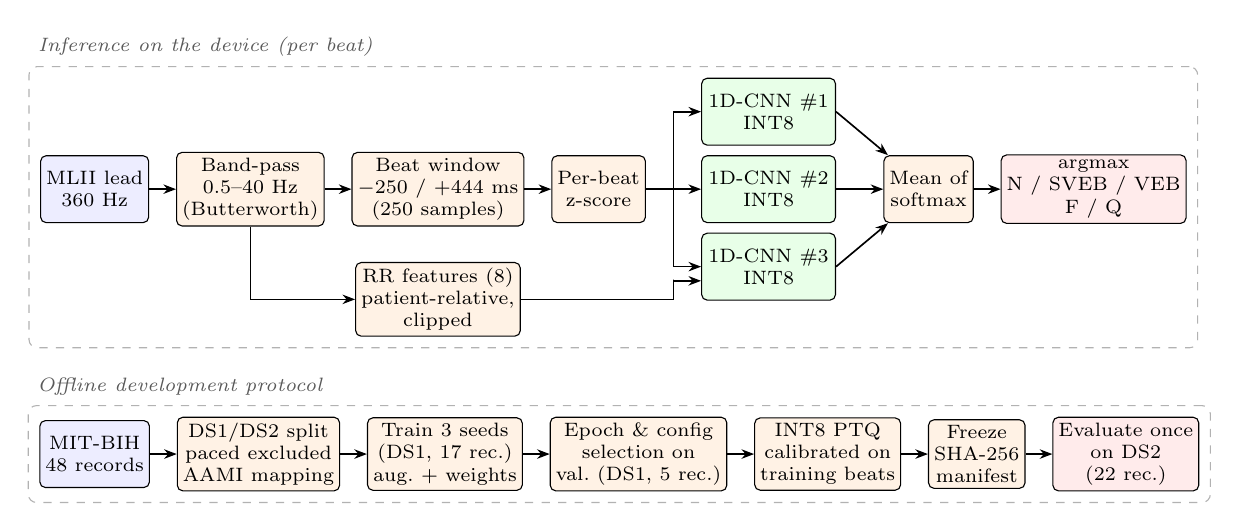
\begin{tikzpicture}[node distance=3.5mm and 3.4mm]
\node[sDATA] (ecg) {MLII lead\\360 Hz};
\node[sPROC, right=of ecg] (bp) {Band-pass\\0.5--40 Hz\\(Butterworth)};
\node[sPROC, right=of bp] (seg) {Beat window\\$-$250 / +444 ms\\(250 samples)};
\node[sPROC, right=of seg] (z) {Per-beat\\z-score};
\node[sPROC, below=of seg, yshift=-1mm] (rr) {RR features (8)\\patient-relative,\\clipped};
\node[sNET, right=7mm of z, minimum width=17mm] (m2) {1D-CNN \#2\\INT8};
\node[sNET, above=1.2mm of m2, minimum width=17mm] (m1) {1D-CNN \#1\\INT8};
\node[sNET, below=1.2mm of m2, minimum width=17mm] (m3) {1D-CNN \#3\\INT8};
\node[sPROC, right=6mm of m2] (avg) {Mean of\\softmax};
\node[sOUT, right=of avg] (cls) {argmax\\N / SVEB / VEB\\F / Q};
\draw[arr] (ecg) -- (bp);
\draw[arr] (bp) -- (seg);
\draw[arr] (seg) -- (z);
\draw[arr] (bp.south) |- (rr.west);
\coordinate (fan) at ($(z.east)!0.5!(m2.west)$);
\draw[arr] (z.east) -- (fan) |- (m1.west);
\draw[arr] (fan) -- (m2.west);
\draw[arr] (fan) |- (m3.west);
\draw[arr] (rr.east) -| ($(fan)+(0,-11.5mm)$) |- ($(m3.west)+(0,-1.8mm)$);
\draw[arr] (m1.east) -- (avg);
\draw[arr] (m2.east) -- (avg);
\draw[arr] (m3.east) -- (avg);
\draw[arr] (avg) -- (cls);
\begin{scope}[on background layer]
\node[lane, fit=(ecg)(cls)(m1)(m3)(rr)] (lane1) {};
\end{scope}
\node[lanelabel] at (lane1.north west) {Inference on the device (per beat)};
\node[sDATA, below=25mm of ecg] (db) {MIT-BIH\\48 records};
\node[sPROC, right=of db] (split) {DS1/DS2 split\\paced excluded\\AAMI mapping};
\node[sPROC, right=of split] (train) {Train 3 seeds\\(DS1, 17 rec.)\\aug.\ + weights};
\node[sPROC, right=of train] (sel) {Epoch \& config\\selection on\\val.\ (DS1, 5 rec.)};
\node[sPROC, right=of sel] (ptq) {INT8 PTQ\\calibrated on\\training beats};
\node[sPROC, right=of ptq] (frz) {Freeze\\SHA-256\\manifest};
\node[sOUT, right=of frz] (ds2) {Evaluate once\\on DS2\\(22 rec.)};
\foreach \a/\b in {db/split, split/train, train/sel, sel/ptq, ptq/frz, frz/ds2} \draw[arr] (\a) -- (\b);
\begin{scope}[on background layer]
\node[lane, fit=(db)(ds2)] (lane2) {};
\end{scope}
\node[lanelabel] at (lane2.north west) {Offline development protocol};
\end{tikzpicture}
\caption{Block diagram. Top: per-beat inference with a three-member INT8 ensemble; the beat and its RR features feed every member. Bottom: development protocol; DS2 is used only after the model is frozen.}
\label{fig:system}
\end{figure*}

\subsection{Dataset and Inter-Patient Protocol}
We use the MIT-BIH Arrhythmia Database~\cite{moody2001impact,goldberger2000physiobank}, downloaded from PhysioNet and verified against its published SHA-256 checksums. Paced records 102, 104, 107 and 217 are excluded. Symbols are mapped to AAMI classes as N\,=\,\{N, L, R, e, j\}, SVEB\,=\,\{A, a, J, S\}, VEB\,=\,\{V, E\}, F\,=\,\{F\} and Q\,=\,\{/, f, Q\}~\cite{aami2012ec57}. Records follow the DS1/DS2 split of~\cite{dechazal2004automatic}. Five DS1 records (106, 118, 201, 220, 223), chosen so that SVEB, VEB and F all occur, form a patient-wise validation set used for every design decision (Table~\ref{tab:data}). Our beat counts match the reference counts of~\cite{dechazal2004automatic} to within 0.1\%.

\begin{table}[t]
\caption{Data Splits and Beat Counts per AAMI Class}
\label{tab:data}
\centering
\footnotesize
\setlength{\tabcolsep}{2.6pt}
\begin{tabular}{@{}lrrrrrrr@{}}
\toprule
Split & Rec. & Beats & N & SVEB & VEB & F & Q \\
\midrule
Train (DS1) & 17 & 40,066 & 36,527 & 552 & 2,581 & 398 & 8 \\
Validation (DS1) & 5 & 10,911 & 9,297 & 391 & 1,207 & 16 & 0 \\
Test (DS2) & 22 & 49,668 & 44,218 & 1,836 & 3,219 & 388 & 7 \\
\bottomrule
\end{tabular}
\end{table}

\subsection{Preprocessing and RR-Interval Features}
The MLII lead is filtered by a fourth-order zero-phase Butterworth band-pass (0.5--40~Hz) to remove baseline wander and noise. Around each annotated R-peak $r$ we take the window $[r-90, r+160)$ (250 samples, about 250~ms before and 444~ms after the peak) and normalize it as $\tilde{\mathbf{x}}=(\mathbf{x}-\mu_{\mathbf{x}})/(\sigma_{\mathbf{x}}+\epsilon)$.

SVEB beats look almost normal but arrive early. With beat times $t_i$ we compute $RR^{\mathrm{pre}}_i=t_i-t_{i-1}$ and $RR^{\mathrm{post}}_i=t_{i+1}-t_i$. We also compute the mean $\overline{RR}^{\mathrm{loc}}_i$ of the previous 10 intervals and the mean $\overline{RR}^{\mathrm{long}}_i$ over the previous 5~min. The eight RR inputs are these four intervals and the ratios
\begin{equation}
\frac{RR^{\mathrm{pre}}_i}{\overline{RR}^{\mathrm{long}}_i},\;
\frac{RR^{\mathrm{post}}_i}{\overline{RR}^{\mathrm{long}}_i},\;
\frac{\overline{RR}^{\mathrm{loc}}_i}{\overline{RR}^{\mathrm{long}}_i},\;
\frac{RR^{\mathrm{pre}}_i}{RR^{\mathrm{post}}_i},
\end{equation}
which compare each beat with the patient's own rhythm (Fig.~\ref{fig:rr}). Gaps in the annotations produce apparent intervals of up to 100~s. These stretched the INT8 input range to 0--11.24 in steps of 0.044, too coarse to resolve prematurity. We therefore clip intervals to 0.2--2.0~s and ratios to 0--3, which gives a step of 0.012. A normalization layer inside the model stores the training mean and variance of the RR inputs.

\begin{figure}[t]
\centering
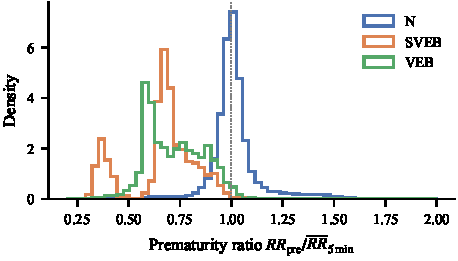
\includegraphics[width=\columnwidth]{rr_prematurity}
\caption{Prematurity ratio on the training set: SVEB and VEB beats arrive early relative to the patient's 5-min mean.}
\label{fig:rr}
\end{figure}

\subsection{Network and Training}
Each ensemble member (Table~\ref{tab:arch}) has two branches. The morphology branch has three blocks of Conv1D (8, 16 and 32 filters; kernels 7, 5 and 5), batch normalization, ReLU and max-pooling by 2, followed by global average pooling. The timing branch normalizes the RR inputs. The branches are concatenated and pass through a 32-unit ReLU layer, dropout of 0.2 and a five-way softmax.

Imbalance is handled with loss weights $w_c=\min\big((N/(K n_c))^{p},\,25\big)$, where $n_c$ is the number of training beats of class $c$, $K=5$, and the exponent $p$ is selected on validation. Training uses Adam~\cite{kingma2015adam} (learning rate $2\times10^{-3}$, batch size 256) with cosine decay~\cite{loshchilov2017sgdr} for up to 60 epochs. Augmentation applies five transformations: amplitude scaling ($\times$0.8--1.2), Gaussian noise, a random baseline drift, a time shift of $\pm$5 samples, and a joint rescaling of the RR intervals ($\times$0.85--1.15). The best epoch is chosen by validation macro-F1 over N, SVEB and VEB; F (16 validation beats) and Q (none) are too rare to select on. Each configuration is trained with three seeds.

\begin{table}[t]
\caption{Layers of One Ensemble Member}
\label{tab:arch}
\centering
\footnotesize
\begin{tabular}{@{}lrr@{}}
\toprule
Layer & Output & Params \\
\midrule
Conv1D(8, $k$=7), BN, ReLU, pool & 125$\times$8 & 56 + 32 \\
Conv1D(16, $k$=5), BN, ReLU, pool & 62$\times$16 & 640 + 64 \\
Conv1D(32, $k$=5), BN, ReLU, pool & 31$\times$32 & 2,560 + 128 \\
Global average pooling & 32 & 0 \\
RR normalization (stored stats) & 8 & 17 \\
Concat, Dense(32), ReLU, dropout & 32 & 1,312 \\
Dense(5), softmax & 5 & 165 \\
\midrule
Total (trainable) & & 4,974 (4,845) \\
\bottomrule
\end{tabular}
\end{table}

\subsection{Quantization, Ensemble and Evaluation}
Each member is quantized to full INT8 by post-training quantization (PTQ)~\cite{jacob2018quantization} calibrated on 2,000 training beats. We also tested quantization-aware training (QAT) with batch normalization folded into the convolutions. Multiply-accumulates (MACs) are counted from the converted graph. Peak activation memory is the largest total size of simultaneously live tensors in execution order, a lower bound on the TensorFlow Lite Micro~\cite{david2021tflm} arena. The ensemble averages the members' dequantized softmax outputs~\cite{lakshminarayanan2017ensembles}. On a microcontroller the members run one after another in the same arena, so peak RAM stays that of one member. Following EC57 we report gross per-class $\mathrm{Se}=TP/(TP+FN)$, $+P=TP/(TP+FP)$ and $\mathrm{FPR}=FP/(FP+TN)$. The model-selection rule was fixed before the candidates' validation results were seen, and the chosen model was frozen with a SHA-256 manifest before its single DS2 evaluation.

\begin{algorithm}[t]
\caption{Per-beat inference on the device}
\label{alg:infer}
\small
\begin{algorithmic}[1]
\Require ECG stream $x$ (MLII, 360 Hz); frozen INT8 members $f_1,\dots,f_M$
\ForAll{detected R-peaks $r_i$}
  \State $\mathbf{b} \gets \mathrm{bandpass}(x)[r_i-90 : r_i+160]$
  \State $\mathbf{b} \gets (\mathbf{b}-\mu_{\mathbf{b}})/(\sigma_{\mathbf{b}}+\epsilon)$
  \State $\mathbf{f} \gets$ 4 RR intervals and 4 ratios of beat $i$, clipped
  \For{$m = 1$ \textbf{to} $M$}
    \State $\mathbf{p}_m \gets \mathrm{dequant}\big(f_m(\mathrm{quant}(\mathbf{b}), \mathrm{quant}(\mathbf{f}))\big)$
  \EndFor
  \State $\hat{y}_i \gets \arg\max_c \frac{1}{M}\sum_{m} \mathbf{p}_m(c)$ \Comment{N, SVEB, VEB, F, Q}
\EndFor
\end{algorithmic}
\end{algorithm}

\begin{algorithm}[t]
\caption{Development and evaluation protocol}
\label{alg:dev}
\small
\begin{algorithmic}[1]
\Require MIT-BIH records; seeds $S=\{0,1,2\}$; candidate configurations $\Theta$
\State Drop paced records; map symbols to AAMI classes
\State Train $\gets$ DS1 $\setminus$ Val; \ Val $\gets$ 5 DS1 records; \ Test $\gets$ DS2
\ForAll{$\theta \in \Theta$, $s \in S$}
  \State Train $f_{\theta,s}$ on Train (weights $w_c$, augmentation, cosine LR)
  \State Keep the epoch with best F1$_{\mathrm{N,S,V}}$ on Val; stop after 15 idle epochs
\EndFor
\State $\theta^\star \gets \arg\max_\theta$ F1$_{\mathrm{N,S,V}}$ on Val \Comment{rule fixed in advance}
\State $q_s \gets \mathrm{PTQ}(f_{\theta^\star,s})$ calibrated on Train, for all $s \in S$
\State Freeze $\{q_s\}$ with a SHA-256 manifest
\State Evaluate the ensemble of $\{q_s\}$ \textbf{once} on Test
\end{algorithmic}
\end{algorithm}

%=====================================================================
\section{Results}
%=====================================================================
\subsection{Model Selection on Validation}
Table~\ref{tab:sweep} summarizes the sweep. Balanced weights ($p=1$) scored best. Augmentation cut the seed-to-seed spread from $\pm$2.48 to $\pm$0.10, and RR clipping raised SVEB sensitivity from 60.6\% to 65.4\%. The final configuration is $p=1$ with augmentation and clipping.

\begin{table}[t]
\caption{Validation Sweep (Mean $\pm$ SD over Three Seeds, \%)}
\label{tab:sweep}
\centering
\footnotesize
\setlength{\tabcolsep}{2.4pt}
\resizebox{\ifdim\width>\columnwidth\columnwidth\else\width\fi}{!}{%
\begin{tabular}{@{}cccccccc@{}}
\toprule
$p$ & Aug. & Clip & F1$_{\mathrm{N,S,V}}$ & SVEB Se & SVEB +P & VEB Se & VEB +P \\
\midrule
0.5 & & & 74.94$\pm$1.26 & 49.7$\pm$14.6 & 40.8 & 85.7 & 89.0 \\
0.5 & \cmark & & 74.71$\pm$1.79 & 54.7$\pm$6.3 & 35.8 & 85.3 & 89.4 \\
0.75 & \cmark & & 75.62$\pm$2.46 & 51.4$\pm$5.0 & 40.1 & 86.4 & 89.8 \\
1.0 & & & 77.06$\pm$2.48 & 52.7$\pm$10.7 & 45.3 & 85.1 & 91.8 \\
1.0 & \cmark & & 76.10$\pm$0.10 & 60.6$\pm$5.5 & 35.0 & 85.6 & 91.3 \\
\textbf{1.0} & \cmark & \cmark & \textbf{77.03$\pm$0.85} & \textbf{65.4$\pm$7.5} & 37.1 & 86.7 & 91.5 \\
\bottomrule
\end{tabular}}
\end{table}

\subsection{Inter-Patient Test Results}
Table~\ref{tab:final} and Fig.~\ref{fig:cm} show the frozen INT8 ensemble on DS2. VEB is detected reliably (Se 92.89\%, +P 92.71\%, FPR 0.51\%). SVEB sensitivity is 74.46\%, but only one SVEB call in three is correct. F beats are not recognized: 372 of the 398 F training beats come from a single patient (record 208), so the model learns that patient rather than fusion morphology. Table~\ref{tab:ensemble} shows that the ensemble beats the mean single member on every listed metric, and it replaces an SVEB sensitivity that varies by $\pm$14 points across seeds with one deterministic result.

\begin{table}[t]
\caption{Frozen INT8 Ensemble on DS2 (Inter-Patient, \%)}
\label{tab:final}
\centering
\footnotesize
\begin{tabular}{@{}lrrrr@{}}
\toprule
Class & Beats & Se & +P & FPR \\
\midrule
N & 44,218 & 88.21 & 97.77 & 16.33 \\
SVEB & 1,836 & 74.46 & 33.43 & 5.69 \\
VEB & 3,219 & 92.89 & 92.71 & 0.51 \\
F & 388 & 0.00 & 0.00 & 4.98 \\
Q & 7 & 0.00 & 0.00 & 0.02 \\
\bottomrule
\end{tabular}
\\[2pt]\parbox{\columnwidth}{\centering\footnotesize Accuracy 87.30, macro-F1 (N, SVEB, VEB, F) 57.92}
\end{table}

\begin{figure}[t]
\centering
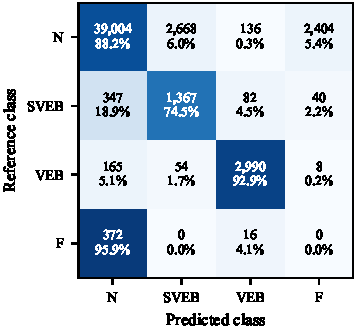
\includegraphics[width=0.72\columnwidth]{confusion_ds2}
\caption{DS2 confusion matrix of the frozen INT8 ensemble (counts and row percentages; Q omitted, 7 beats).}
\label{fig:cm}
\end{figure}

\begin{table*}[t]
\caption{Single Members (Mean $\pm$ SD, $n=3$) Versus the Ensemble on DS2 (\%)}
\label{tab:ensemble}
\centering
\footnotesize
\begin{tabular}{@{}lcccccccc@{}}
\toprule
Model & Accuracy & Macro-F1 & N Se & N FPR & SVEB Se & SVEB +P & VEB Se & VEB +P \\
\midrule
FP32, single & 85.72$\pm$2.52 & 56.72$\pm$0.45 & 86.46$\pm$2.78 & 15.74$\pm$3.03 & 76.33$\pm$12.96 & 31.46$\pm$1.76 & 91.44$\pm$4.05 & 90.88$\pm$2.84 \\
FP32, ensemble & 87.39 & 58.25 & 88.04 & 14.07 & 80.99 & 33.65 & 92.85 & 92.48 \\
INT8, single & 85.70$\pm$2.73 & 56.31$\pm$0.63 & 86.66$\pm$3.02 & 17.73$\pm$2.88 & 71.11$\pm$13.98 & 30.93$\pm$1.26 & 91.27$\pm$3.96 & 90.73$\pm$3.08 \\
\textbf{INT8, ensemble (final)} & \textbf{87.30} & \textbf{57.92} & \textbf{88.21} & \textbf{16.33} & \textbf{74.46} & \textbf{33.43} & \textbf{92.89} & \textbf{92.71} \\
\bottomrule
\end{tabular}
\end{table*}

\subsection{Quantization and Embedded Feasibility}
INT8 shrinks the weights of one member 3.7$\times$ (18.8 to 5.0~KB) and its peak activation memory 4$\times$ (15.7 to 3.9~KB), at a cost of 0.5--0.6 points of accuracy (Table~\ref{tab:quant}). QAT matched FP32 on validation before fine-tuning, so it brought no accuracy gain. The only noticeable quantization cost is SVEB sensitivity (81.0\% to 74.5\% for the ensemble). The ensemble's activations use about 0.8\% of the ESP32-WROOM-32E's 520~KB SRAM, and its files about 1.4\% of 4~MB flash. Assuming 10 cycles per MAC (to be verified on hardware), inference would take about 32~ms per beat at 240~MHz, about 4\% of the beat interval at 75~bpm. Kim et al.~\cite{kim2024ultraedge}, by comparison, report 118~kB RAM.

\begin{table}[t]
\caption{Model Cost and DS2 Accuracy Before and After Quantization}
\label{tab:quant}
\centering
\footnotesize
\setlength{\tabcolsep}{2.5pt}
\resizebox{\ifdim\width>\columnwidth\columnwidth\else\width\fi}{!}{%
\begin{tabular}{@{}lrrrrrr@{}}
\toprule
Model & File & Weights & MACs & Peak act. & Acc. & SVEB \\
 & (KB) & (KB) & (k) & (KB) & (\%) & Se (\%) \\
\midrule
FP32 (1 member) & 28.9 & 18.8 & 254 & 15.7 & 83.46 & 78.38 \\
INT8 PTQ (1 member) & 18.6 & 5.0 & 254 & 3.9 & 82.83 & 72.06 \\
INT8 QAT (1 member) & 13.8 & 5.0 & 254 & 2.9 & 82.97 & 72.28 \\
\textbf{INT8 PTQ ensemble} & \textbf{55.9} & \textbf{15.1} & \textbf{762} & \textbf{3.9} & \textbf{87.30} & \textbf{74.46} \\
\bottomrule
\end{tabular}}
\end{table}

\subsection{Error Analysis and Ablations}
Of the 2,668 normal beats called SVEB, 86.5\% come from five of the 22 test patients (Fig.~\ref{fig:fa}). Their rhythm annotations show atrial fibrillation (AF) or flutter in four of them (37--97\% of beats) and 2:1 AV block in the fifth. In AF the rhythm is irregular throughout, so normal beats often arrive early, which the model has learned to associate with SVEB. These errors are confident (mean SVEB probability 0.78). A validation-tuned SVEB threshold therefore gained only 0.15 points on validation, and we kept plain argmax.

\begin{figure}[t]
\centering
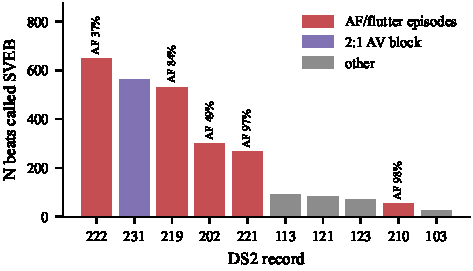
\includegraphics[width=\columnwidth]{false_alarms_by_record}
\caption{Normal beats misclassified as SVEB, by DS2 record (ten largest), with the share of beats inside AF/flutter episodes from the MIT-BIH rhythm annotations.}
\label{fig:fa}
\end{figure}

We then added two rhythm-irregularity inputs (``+Irreg.''), with global max pooling. These are the coefficient of variation and the mean successive difference of the ten RR intervals \emph{preceding} each beat. A ``causal'' variant also drops every input that needs the next beat. The pre-declared validation rule selected the original model (Table~\ref{tab:ablation}). On DS2, however, +Irreg.\ raises SVEB +P from 33.43\% to 42.31\% and macro-F1 by 2.8 points. Our validation set has no AF patient, so it could not reward this feature. Selecting it now would mean choosing on the test set, so we report it as an ablation only. The causal variant mislabels 7,242 normal beats as F.

\begin{table}[t]
\caption{Ablations (INT8 Ensembles; Validation Selects, DS2 Reports, \%)}
\label{tab:ablation}
\centering
\footnotesize
\setlength{\tabcolsep}{2.2pt}
\resizebox{\ifdim\width>\columnwidth\columnwidth\else\width\fi}{!}{%
\begin{tabular}{@{}lccccccr@{}}
\toprule
 & Val. & \multicolumn{5}{c}{DS2} & Wts. \\
\cmidrule(lr){2-2}\cmidrule(lr){3-7}
Model & F1$_{\mathrm{N,S,V}}$ & mF1 & S Se & S +P & V +P & N Se & (KB) \\
\midrule
\textbf{Frozen (selected)} & \textbf{77.60} & 57.92 & 74.46 & 33.43 & 92.71 & 88.21 & 15.1 \\
+Irreg.\ +max-pool & 74.76 & 60.75 & 77.72 & 42.31 & 91.83 & 89.64 & 18.3 \\
Causal +Irreg. & 76.00 & 57.93 & 78.10 & 39.56 & 86.64 & 78.02 & 18.0 \\
\bottomrule
\end{tabular}}
\end{table}

\subsection{Comparison and Limitations}
On SVEB our sensitivity matches de Chazal et al.~\cite{dechazal2004automatic} (75.9\%) but our +P is lower (33.4\% vs.\ 38.5\%). On VEB our model is clearly stronger (92.9/92.7\% vs.\ 77.7/81.9\%). Among studies with embedded evidence (Table~\ref{tab:e3c}), ours is the only one that combines the canonical inter-patient split with a microcontroller-class memory footprint. DS2 was evaluated seven times during development. One design change followed a DS2 observation: the quantization comparison exposed the RR-range problem, fixed by clipping, which also raised validation SVEB sensitivity by 4.8 points. Every other choice was made on validation. Further limitations are that records 201 (validation) and 202 (DS2) come from the same patient, that we use reference R-peak annotations, and that embedded costs are estimated from the converted graphs rather than measured on the device.

%=====================================================================
\section{Conclusion}
%=====================================================================
We presented a three-member INT8 1D-CNN ensemble for five-class AAMI heartbeat classification that meets all three E3C criteria. On unseen patients it detects 92.9\% of ventricular and 74.5\% of supraventricular ectopic beats with 15.1~KB of weights and about 4~KB of working memory, and quantization costs almost no accuracy. SVEB false alarms are concentrated in atrial-fibrillation patients. A rhythm-irregularity feature reduces them, but its benefit is visible only with AF patients in the validation data. Future work will rebuild the validation protocol with AF records before re-selecting, deploy the frozen model with TensorFlow Lite Micro on an ESP32-WROOM-32E to measure latency, memory and energy, and add an on-device R-peak detector.

\bibliographystyle{IEEEtran}
\bibliography{refs}

\end{document}
